\documentclass[10pt, letterpaper, titlepage]{article}
% \documentclass[10pt, letterpaper, titlepage]{report}

% % Packages
\input{../../packages.tex}
\input{../../commands.tex}

% Problem 5
\usepackage{tikz}
\usetikzlibrary{fit,shapes}

% % Change lable to letter from number
% \renewcommand{\thesubsection}{\alph{subsection}}

% Paragraph setup
\usepackage{parskip}
\setlength\parindent{0pt}

% Size of section header
\usepackage{sectsty}
\chaptertitlefont{\fontsize{17}{0}\selectfont}
\sectionfont{\fontsize{11}{13}\selectfont}
\subsectionfont{\fontsize{10}{12}\selectfont}
\subsubsectionfont{\fontsize{10}{12}\selectfont}

\usepackage{hyperref} % Doesn't like math in section titles
\newcommand{\smath}[2]{\texorpdfstring{#1}{#2}} % Use this to not break hyperref
% \section[title in bookmark]{title} % also works
% I did'nt find this out until half way through this assignment

% \setcounter{secnumdepth}{-1} % Sets sectioning level for numbering 
% % -1 part     1 section     3 subsubsection  5 subparagraph
% %  0 chapter  2 subsection  4 paragraph

% % Debug
% % For \hbox too wide errors.
% \overfullrule=.01cm

% Header
\geometry{margin = 1in}
\pagestyle{fancy}
% \pagenumbering{gobble} % Removes page number
\headheight = 23.01503pt
\lhead{}
\rhead{Yifeng Pan
     \\UCID: 30063828}

% Title page
\title{MATH 315 Assignment 2}
\author{Instructor: Dr. Thomas Bitoun
    \\Name: Yifeng Pan
    \\UCID: 30063828}
\date{Winter 2020}

\begin{document}
    \maketitle

    \section[Problem 1]{
}  
    \subsection[(i)]{Let $C_{15}$ be a cyclic group of order $15$. 
        How many subgroups does $C_{15}$ have? List all of them.
    }
        Let $g$ be a generator of $C_{15}$.

        The order of every subgroup of $C_{15}$ has to divide $15$.

        The divisors of $15$ are $\set{1,3,5,15}$.
        So the subgroups of $C_{15}$ can be generated using $g^1, g^3, g^5, g^{15}$.

        The subgroups are:
        \begin{align*}
                C_{15} &= \set{g^0 = g^{15}, g^1, g^2 , \hdots, g^{14}}, \\
                C_{5} &= \set{g^0 = g^{3^5}, g^{3}, g^{3^2}, g^{3^3}, g^{3^4}}, \\
                C_{3} &= \set{g^0 = g^{5^3}, g^{5}, g^{5^2}}, \\
                C_{1} &= \set{g^0}
        \end{align*}

    \subsection[(ii)]{Give an example of a simple group of order $60$.
        (You do not need to justify your answer for part (ii).)
    }
        % Since every simple group of order $60$ is isomorphic to the alternating group $A_5$,
        % $A_5$ itself must be an simple group.
        $A_5$ is the archetypical simple group,
        where every simple group of order $60$ is isomorphic to $A_5$.
    \newpage
    \section[Problem 2]{Let $a \in R$, where $R$ is a commutative ring.
    Let $R[x]$ be the ring of polynomials over $R$.}
    \subsection[(i)]{Show that the factor ring $R[x]/(x-a)$, where $(x-a)$ is the principal
        ideal generated by $x-a\in R[x]$, is isomorphic to the ring $R$.
    }
        \footnote{Reference: “Algebra” by Michael Artin, Section 11.4, Quotient Rings.}
        % We define a surjective ring homomorphism $f: R[x] \to R$, such that $(x-a) = \ker(f)$.
        Let $f: R[a] \to R$ be a ring homomorphism.

        Since $(x-a)$ contains all multiples of $x - a$,
        we know $\lall i \in (x-a), f(i) = 0$.
        Now, suppose $i \not\in (x-a)$. 
        Then $a$ is not a factor of $i$, and $f(i) \neq 0$.
        Therefore $(x-a) = \ker(f)$.

        Now, Let $r \in R \subset R[x]$.
        Since $f(r) = r$, $f$ is surjective.

        Since $f$ is surjective, and $(x-a) = \ker(f)$: \\
        By the First Isomorphism Theorem, $\overline{f}: R[x] / (x-a) \to R$ is an isomorphism.
        \qed


    \subsection[(ii)]{Let $R' = R[x]/(ax-1)$ and let $u = [x]$ be the class of $x$ in $R'$.
        Show that every element $y$ of $R'$ can be written as $y = u^lr$, where $l \geq 0$
        and $r$ is the class of a constant polynomial i.e. the class in $R'$ of an element 
        of $R$.}
        % \footnote{\url{https://math.stackexchange.com/questions/1996936/the-kernel-of-the-quotient-map-r-to-rx-ax-1}}
        % \footnote{\url{https://math.stackexchange.com/questions/2121605/let-a-be-an-element-of-a-ring-r-let-r-be-the-ring-rx-ax-1-show-that-every}}
        % Let $I = (ax-1)$, where $a \in R$.

        % % $R[x]/(ax-1)$ is the factor ring obtained from $R[x]$ by killing $ax - 1$.

        % Let $u = [x] = x + I$.

        % We have $u^l = (x+I)^l = x^l + I = [x^l]$.

        % Let $c \in R$,
        % and $r = [c] = c + I$.

        % So $u^lr = (x^l + I)(c + I) = x^lc + I = [cx^l]$.

        % It is sufficint to prove $R[x]/(ax -1) = \set{[cx^l] | c\in R, l \geq 0}$.

        % Let $f(x) \in R[x]$.



        % Let $y \in R' = R[x]/I$.

        % Let $y'$ be in the class of $y$.

        % We need to prove $\lis c \in R, l \in \N\union \set{0}, z\in R[x]$ 
        % such that $y' = cx^l + I = cx^l + zax - z$.

        % Attempt 2
        % Define a surjective ring homomorphism $\phi: R[x] \to R[x]/(ax-1)$,
        % where $\ker(\phi) = (ax-1)$.

        % Let $I = (ax-1)$.

        % $u = \phi(x) = x + I$.



    \subsection[(iii)]{For which positive integers $n$ does $x^2+x+1$ divide $x^4+3x^3+x^2+7x+5$
        in the ring of polynomials over $\Z / n\Z$? Justify your answers.}

        % We have $\Z / n \Z [x]$.

        We have $(x^2 + x +1)(ax^2 + bx + c) = (x^4 + 3x^3 + x^2 + 7x+5)$ in $\Z/n\Z[x]$ 
        for some $a,b,c\in \Z/n\Z$.

        This gives 
        \begin{align*}
            a &\cmod{1}{n} \\
            a + b &\cmod{3}{n} \\
            a + b + c &\cmod{1}{n} \\
            b + c &\cmod{7}{n} \\
            c &\cmod{5}{n} \\
            &\downarrow \\
            a &\cmod{1}{n} \\
            b &\cmod{2}{n} \\
            c &\cmod{5}{n} \\
            a + b + c &\cmod{1}{n} \\
            &\downarrow \\
            1 + 2 + 5 &\cmod{1}{n} \\
            &\downarrow \\
            7 &= kn \text{ for some $k,n \in \Z$.}
        \end{align*}

        So $n \in \set{1,7}$.
        \qed
    \newpage
    \section[Problem 3]{Let $n$ be the natural number $\in\set{1,2,3,\hdots}$.
    An $n$th root of unity is a complex number $z$ such that $z^n = 1$.}
    \subsection[(i)]{Prove that the $n$th roots of unity form a cyclic subgroup 
        $H_n$ of $\C^\times$ of order $n$.
        (Recall that $\C^\times = \C - \set{0}$, with the complex multiplication.)}

        Let $n \in \set{1,2,3,\hdots} = \N$.
        Let $Z_n = \set{z | z \in \C \land z^n = 1}$.
        Let the group $H_n$ be $Z_n$ under complex multiplication.
        Since there are $n$ solution to $z \in \C, z^n = 1$,
        the order of $H_n$ is $n$.

        $H_n$ inherits associativity from $\C^\times$.

        $H_n$ contains the identity $1$, as $1^n = 1, \lall n \in \N$.

        Let $a,b \in H_n$. Now, $(ab)^n = a^nb^n = 1 \times 1 = 1$.
        Therefore $ab \in H_n$, and $H_n$ is closed.

        Let $a \in H_n$. $a^{n-1}$ is the inverse,
        as $aa^{n-1} = a^{n-1}a = a^n = 1$.
        Now, $\left(a^{n-1}\right)^n = \left(a^n\right)^{n-1} = 1^{n-1} = 1$.
        Therefore every element of $H_n$ has an inverse in $H_n$.

        Therefore $H_n$ is a subgroup of $\C^\times, \lall n \in \N$.
        \qed
        
        Now, since all elements of $H_n$ are on the unit circle on the complex plane centered at $(0,0)$,
        all elements of $H_n$ can be written in the form $\exp(ix)$.
        (Assume reduced form where $x = x\mod 2\pi$.
            % \footnote{Define an equivelence class where $\exp(ia) = \exp(ib) \liff$}
        )

        Let $n \geq 2$. ($n = 1$ is the trivial case.)

        Let $m = \exp(ix) |( x \neq 0 \land \exp(ix) \in H_n) \land \lall \exp(iy) \in H_n, x \leq y$.
        (If $m$ is not unique, then $H_n$ is not a set. Therefore $m$ is unique.)

        Let $Y_n$ be the cyclic subgroup generated from $m \in \C^\times$.

        Let $y \in Y_n$.
        So $y = m^z$ for some $z \in \Z$.
        Now, since $m \in H_n$, $y^n = m^{z^n} = m^{n^z} = 1^z = 1$.
        Therefore $y \in H_n$.

        Now we find the order of $Y_n = \abs{\set{m^{0}, m^1, m^{-1}, m^2, m^{-2}, \hdots}}$.
        Let $z \in Z$.
        Let $z = qn + r | q \in \Z, r \in [0,n) \intersection \Z$. (The solution to $q,r$ is unique.)

        Now $m^z = m^{qn} m^r = 1^q m^r = m^r$.
        Therefore $Y_n = \set{m^0, m^1, m^2, \hdots, m^{n-1}} = \set{m^r}$.

        Now we prove $m^0, \hdots, m^{n-1}$ are distinct.
        Due to the cancellation law derived from the inverse property of groups,
        it is sufficient to prove that $m^0 \neq m^k, \lall 0 < k < n, k \in \N$.

        By contradiction:
        Suppose $\lis k \in (0,n) \intersection \N$
        , where $m^k = 1$.
        % So $\exp(\frac{ixkn}{n}) = \exp(ix k) = m^k = 1$.
        Since $\exp(i\frac{xk}{n})^n = \exp(\frac{ixkn}{n}) = \exp(ix k) = m^k = 1$,
        therefore $\exp(i\frac{xk}{n}) \in H_n$.
        Since $\frac{k}{n} < 1$,
        $x > \frac{xk}{n}$.
        This is a contradiction from the construction of $x$.
        Therefore there exists no such $m^k$.

        Therefore $m^0, \hdots, m^{n-1}$ are distinct,
        and $\abs{Y_n} = n$.
        
        Therefore $Y_n$ and $H_n$ have the same order,
        and since $Y_n \subseteq H_n, Y_n = H_n$.

        Therefore $H_n$ is a cyclic subgroup of $\C^\times$.
        \qed


    \subsection[(ii)]{Determine the product of all the $n$th roots of unity.}
        $-1$ if $n$ is even, $1$ if $n$ is odd. 

        Let $a \in H_n$.
        If $a$ and $a^{-1}$ are distinct elements,
        then they cancel out to the identity.
        The only cases where $a = a^{-1}$ is $a \in \set{1, -1}$.
        We can ignore the identity.
        And $-1 \in H_n \liff n $ is even.

    \newpage
    \subsection[(iii)]{Show that if the only subgroups of $H_n$ are the trivial subgroups 
        $\set{1}$ and $H_n$, then $n = 1$ or $n$ is a prime number.}
        We prove the contrapositive.
        Suppose $n \neq 1$ and $n$ is not prime.
        So $\lis a,b \in \N$ such that $ab = n \geq 4, a > 1, b > 1$.

        (The following two paragraphs are a repeat of (3.1):)

        Now, since all elements of $H_n$ are on the unit circle on the complex plane centered at $(0,0)$,
        all elements of $H_n$ can be written in the form $\exp(ix)$.
        (Assume reduced form where $x = x\mod 2\pi$.)
        
        Let $m = \exp(ix) |( x \neq 0 \land \exp(ix) \in H_n) \land \lall \exp(iy) \in H_n, x \leq y$.
        (If $m$ is not unique, then $H_n$ is not a set. Therefore $m$ is unique.)

        Let $Y_n$ be the cyclic subgroup generated from $m^a \in \C^\times$.

        We've proven in (3.1) that $m^a \neq m^0 = 1$.
        Therefore $Y_n \neq \set{1}$.

        Now we prove $m \not\in Y_n$ by contradiction (Note: $Y_n$ is generated from $m^a$.):
        Suppose $m \in Y_n$.
        So $\lis z \in \Z, m^1 = m^{az}$.
        Therefore $az \cmod{1}{n}$, or $az = kn + 1$ for some $k \in Z$.
        So $az = kab + 1$ and $a(z - kb) = 1$.
        Therefore $a \in \set{-1,1}$,
        which is a contradiction as $a > 1$ by construct.
        Therefore $m \not\in Y_n$.
        Since $m \in H_n$, $Y_n \neq H_n$.

        Therefore if $n \neq 1$ and $n$ is a non-prime, 
        then we can construct $Y_n$ to be a non-trivial subgroup of $H_n$.
    \newpage
    \section[Problem 4]{Let $R$ be a commutative ring.}
    \subsection[(i)]{Assume that the characteristic of $R$ is a prime number $p$.
        Prove that if $r \in R$ is nilpotent i.e. $r^n = 0$ for some $n \geq 0$,
        then there is an $l \geq 1$ such that $(1 + r)^l= 1$.
    }
        % \footnote{\url{https://en.wikipedia.org/wiki/Frobenius_homomorphism}}
        % \footnote{Reference: \url{https://en.wikipedia.org/wiki/Characteristic_(algebra)}.}
        Since the characteristic of $R$ is $p$,
        $\lall r \in R, p r = 0$.
        
        Let $r \in R$.

        % \footnote{Proof: 
        %     \url{https://math.stackexchange.com/questions/2834493/prime-number-rows-in-a-pascals-triangle/2834502\#2834502}.}
        \footnote{\url{https://en.wikipedia.org/wiki/Freshman\%27s_dream\#Prime_characteristic}.}
        We know $(1+r)^p = 1 + r^p$.
        And $(1+r)^{(p^k)} = 1+r^{(p^k)}$.

        \footnote{I got the idea that I needed $p^k \geq n$, not $p^k \cmod{0}{n}$,
            from Devin Kwok (UCID: 10016484).}
        Choose $k$ such that $p^k \geq n$.

        Let $l = p^k$.

        Then $(1+r)^l = 1 + r^l = 1 + r^nr^{l-n} = 1 + 0r^{l-n} = 1$.
        \qed

%         By Euler's Theorem:
%         Since $p$ and $n$ are coprime,
%         $\lis k$ such that $p^k \cmod{1}{n}$.

%         This means $(1 + r)^{(p^k)} = 1 + r^{(p^k)} = 1 + r$.

% (
%         Doesn't work.
%         R is not an integral domain.
% )

%         So $(1 + r)^{(p^k)} - (1 + r) = 0
%         \to (1 + r) ( (1 + r)^{(p^k) - 1} - 1) = 0$.

%         Therefore $(1 + r)^{(p^k) - 1} = 1$.
%         Let $l = p^k - 1$.
        % \qed


    \subsection[(ii)]{Prove that an integral domain of finite order is a field.}
        \footnote{Reference: \url{https://en.wikipedia.org/wiki/Integral_domain}.}
        Let $R = \set{0, r_1, r_2, \hdots, r_{n-1}}$ be an finite integral domain of order $n$.

        We prove the only ideals of $R$ are $(0)$ and $(1)$.

        Let $I$ be an ideal of $R$.

        Suppose $I \neq (0)$.

        Let $i \in I, i \neq 0$.

        Let $J = (i) = \set{ir | r \in R} = \set{0} \union \set{ir_1, ir_2, \hdots, ir_{n-1}}$.

        We prove $ir_1, ir_2, \hdots, ir_{n-1}$ are distinct.

        Suppose $\lis a,b, a \neq b$ such that $ir_a = ir_b$.

        Now, $ir_a = ir_b \to 0 = ir_a - ir_b = i(r_a - r_b)$.

        Since $R$ is an integral domain, and $i \neq 0$, we know
        $r_a - r_b = 0$. Contradiction.

        Therefore $ir_1, ir_2, \hdots, ir_{n-1}$ are distinct,
        and the order of $J$ is $1 + (n - 1) = n$.

        Therefore $I = J = R$.

        Therefore $R$ only has two ideals.

        \footnote{Reference: “Algebra” by Michael Artin, Proposition 11.3.19 (b).}
        Therefore $R$ is a field.
        \qed

    \subsection[(iii)]{Find $x \in \Z$ such that $x = 3$ modulo $8$ and $x = 2$ modulo $5$.}
        \footnote{Reference: \url{https://en.wikipedia.org/wiki/Chinese_remainder_theorem\#Computation}.}
        $5$ and $8$ are coprimes.

        So we only have to check integers between $0$ and $5 * 8 = 45$.

        The solutions to $x \cmod{2}{5}$ are $\set{2,7,12,17,22,27,32,37,42}$.

        The solutions to $x \cmod{3}{8}$ are $\set{3, 11, 19, 27, \hdots}$.

        We found $x = 27$.
    \newpage
    \section[Problem 5]{Recall our notation for the dihedral group $D_n, n \geq 1$.
    We have $x,y\in D_n$ such that the orders $o(x) = n, o(y)=2, yx = x^{-1}y$ and $D_n = <x,y>$.}
    \subsection[(i)]{Write down the element $x^2yx^{-1}y^{-1}x^3y^3$ of $D_n$
        in the form $x^iy^i$, for integers $i,j \geq 0$.}

        We have $x^n = 1, y^2 = 1, yx = x^{-1}y$.
        Now, 
        \begin{align*}
            yx &= x^{-1}y \\
            y &= x^{-1}y x^{-1} \\
            xy &= y x^{-1} \\
            % 
            \to & x^2yx^{-1}y^{-1}x^3y^3 \\
            = & x^2yx^{-1}y^{-1}x^3y \\
            = & x (y x^{-1}) x^{-1}y^{-1}x^2 (y x^{-1}) \\
            = & x y x^{-2}y^{-1}x^2 y x^{-1} \\
            = & y x^{-3}y^{-1} y x^{-3} \\
            = & y x^{-3} x^{-3} \\
            = & y x^{-6} \\
            = & x^6 y \\
            \to & i = 6, j = 1
        \end{align*}


    \subsection[(ii)]{Let $G$ be a group. Show that for all $a\in G$, if the subset $\set{1,a}$
        is a normal subgroup of $G$ then $a$ is in the center of $G$.
        Prove that $N = \set{1, x^5}$ is a normal subgroup of $D_{10}$.}
        
        Suppose $a\in G$ such that $\set{1,a}$ is a normal subgroup of $G$.
        % So $\lall g \in G, gag^{-1} \in \set{1,a}$.

        Let $x \in G$.
        Since $\set{1,a}$ is a normal subgroup of $G, xax^{-1} \in \set{1,a}$.
        If $xax^{-1} = a$, then $xa = ax$, we're done.
        If $xax^{-1} = 1$, then $a = 1$, so $xa = ax$.
        \qed

        % We need to prove $N = \set{1,x^5}$ is a normal subgroup of $D_{10}$.

        We have $x,y \in D_{10}, x^{10} = 1, y^2 = 1, yx = x^{-1}y$.

        Let $h \in N = \set{1,x^5}$. $h = 1$ is the trivial case, so assume $h = x^5$.

        Now, $x x^5 x^{-1} = x^5 \in N$, and $y x^5 y^{-1} = x^{-5} y y^{-1} = x^{-5} = x^5 \in N$.
        And any combination of $x$ and $y$ would yield the same result.
        Therefore $N$ is a normal subgroup of $D_{10}$.
        \qed
        
        

    \subsection[(iii)]{Compute the left cosets of $N$ in $D_{10}$ and show that the quotient group
        $\frac{D_{10}}{N}$ is isomorphic to $D_5$.}

        \(
            \set{
                \set{1, x^5},
                \set{x, x^6},
                \set{x^2, x^7},
                \set{x^3, x^8},
                \set{x^4, x^9},
                \set{y, yx^5},
                \set{yx, yx^6},
                \set{yx^2, yx^7},
                \set{yx^3, yx^8},
                \set{yx^4, yx^9}
            }
        \).

        We find a bijective group homomorphism from $D_{10}/N$ to $D_5$.

        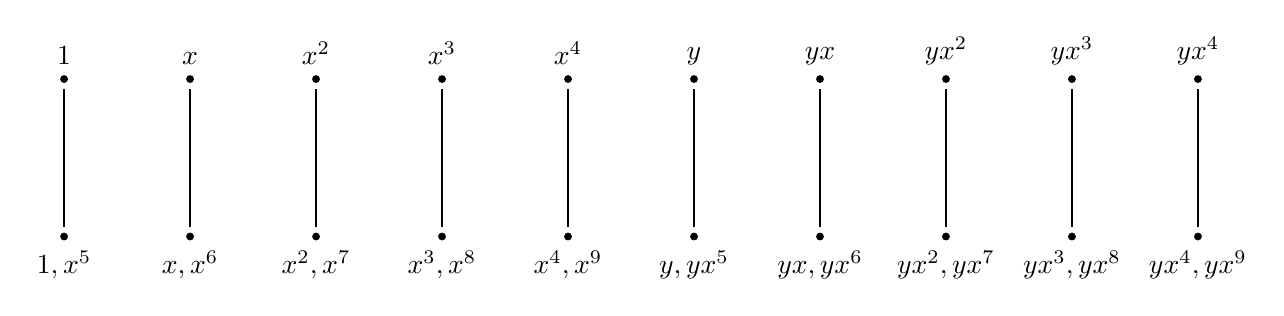
\begin{tikzpicture}[
            ele/.style={fill=black,circle,minimum width=.8pt,inner sep=1pt}
        ]
            \node[ele,label=above:$1$] (b1) at (0,2) {};
            \node[ele,label=above:$x$] (b2) at (1.6,2) {};    
            \node[ele,label=above:$x^2$] (b3) at (3.2,2) {};
            \node[ele,label=above:$x^3$] (b4) at (4.8,2) {};
            \node[ele,label=above:$x^4$] (b5) at (6.4,2) {};
            \node[ele,label=above:$y$] (b6) at (8,2) {};
            \node[ele,label=above:$yx$] (b7) at (9.6,2) {};    
            \node[ele,label=above:$yx^2$] (b8) at (11.2,2) {};
            \node[ele,label=above:$yx^3$] (b9) at (12.8,2) {};
            \node[ele,label=above:$yx^4$] (b10) at (14.4,2) {}; 

            \node[ele,label=below:$\set{1, x^5}$] (a1) at (0,0) {};
            \node[ele,label=below:$\set{x, x^6}$] (a2) at (1.6,0) {};    
            \node[ele,label=below:$\set{x^2, x^7}$] (a3) at (3.2,0) {};
            \node[ele,label=below:$\set{x^3, x^8}$] (a4) at (4.8,0) {};
            \node[ele,label=below:$\set{x^4, x^9}$] (a5) at (6.4,0) {};
            \node[ele,label=below:$\set{y, yx^5}$] (a6) at (8,0) {};
            \node[ele,label=below:$\set{yx, yx^6}$] (a7) at (9.6,0) {};    
            \node[ele,label=below:$\set{yx^2, yx^7}$] (a8) at (11.2,0) {};
            \node[ele,label=below:$\set{yx^3, yx^8}$] (a9) at (12.8,0) {};
            \node[ele,label=below:$\set{yx^4, yx^9}$] (a10) at (14.4,0) {}; 

            \draw[thick,shorten <=2pt,shorten >=2pt] (a1) -- (b1);
            \draw[thick,shorten <=2pt,shorten >=2pt] (a2) -- (b2);
            \draw[thick,shorten <=2pt,shorten >=2pt] (a3) -- (b3);
            \draw[thick,shorten <=2pt,shorten >=2pt] (a4) -- (b4);
            \draw[thick,shorten <=2pt,shorten >=2pt] (a5) -- (b5);
            \draw[thick,shorten <=2pt,shorten >=2pt] (a6) -- (b6);
            \draw[thick,shorten <=2pt,shorten >=2pt] (a7) -- (b7);
            \draw[thick,shorten <=2pt,shorten >=2pt] (a8) -- (b8);
            \draw[thick,shorten <=2pt,shorten >=2pt] (a9) -- (b9);
            \draw[thick,shorten <=2pt,shorten >=2pt] (a10) -- (b10);
        \end{tikzpicture}
        \qed

    \section*{Citations}
    ``Algebra'' by Michael Artin
    (ISBN 13: 9780132413770).

    Proofread by Devin Kwok
    (UCID: 10016484).

\end{document}
